\documentclass[a4paper,12pt]{article}
\usepackage[utf8]{inputenc}
\usepackage[cm,empty]{fullpage}
\usepackage[T2A]{fontenc}
\usepackage[english, russian]{babel}
\usepackage{amssymb,amsmath,amsxtra,amsthm}
\usepackage{proof}
\usepackage[pdftex]{graphicx}
\usepackage{wrapfig}
\usepackage{braket}
\usepackage{xcolor}

\usepackage[left=2cm,right=2cm,
    top=1cm,bottom=1cm,bindingoffset=0cm]{geometry}

\renewcommand{\leq}{\leqslant}
\renewcommand{\geq}{\geqslant}


\newcommand{\iiff}{\Longleftrightarrow}
\renewcommand{\iff}{\Leftrightarrow}
\newcommand{\nothing}{\varnothing}

\newtheorem*{rem}{Замечание}

\newcommand{\NN}{\mathbb{N}}
\newcommand{\ZZ}{\mathbb{Z}}
\newcommand{\Q}{\mathbb{Q}}
\newcommand{\A}{\mathbb{A}}
\newcommand{\R}{\mathbb{R}}
\renewcommand{\C}{\mathbb{C}}

\renewcommand{\phi}{\varphi}
\newcommand{\eps}{\varepsilon}

\makeatletter
\newcommand*{\rom}[1]{\expandafter\@slowromancap\romannumeral #1@}
\makeatother

\newcounter{z}


\newcommand{\zs}{\refstepcounter{z}\vskip 10pt\par\noindent
\fbox{\textbf{12.\arabic{z}}} }

\newcommand{\z}{\refstepcounter{z}\vskip 20pt\noindent
\fbox{\textbf{\arabic{z}}} }

\renewcommand{\date}{{\bf 7 марта 2021}} 

\newcommand{\dif}
{
------------------------------------------------------------------------------------------------------------------------------------------------------
}

\newcommand{\HSEhat}{
\vspace*{-0pt}
\noindent
\setcounter{z}{0}


{\bf \phantom{\date}  \large \hfill Линейная алгебра: \hfill \normalsize \date}

\vspace{5 pt}
{\bf \large \hfill  лекция 1\hfill }

\vspace{15 pt}
\centerline{ \large  Домашнее задание.}
\centerline{ \large  Кирилл Сетдеков}



\vspace*{10pt}
\setcounter{z}{0}

}

\begin{document}
\HSEhat


\subsection*{Задачи}

\begin{enumerate}


\item Решите систему линейных уравнений:
\[
\left\{
\begin{aligned}
&6x + 12y + 5z + t = -6\\
&9x + 18y + 17z -8t = -9\\
&5x + 10y + 4z + t = -5
\end{aligned}
\right.
\]
\textbf{Решение:}\\
Запишем в виде матрицы $Ax=b$


$\left(\begin{array}{cccc|c}  
 6 & 12 & 5 & 1 & -6 \\  
 9 & 18 & 17 & -8 & -9  \\ 
 5 & 10 & 4 & 1 & -5  \\ 
\end{array}\right)
\rightarrow$  вычтем  \rom{1} - \rom{3} 
$\left(\begin{array}{cccc|c}  
 1 & 2 & 1 & 0 & -1 \\  
 9 & 18 & 17 & -8 & -9  \\ 
 5 & 10 & 4 & 1 & -5  \\ 
\end{array}\right)
\rightarrow$ вычтем  \rom{2} - 9(\rom{1})
$\left(\begin{array}{cccc|c}  
 1 & 2 & 1 & 0 & -1 \\  
 0 & 0 & 8 & -8 & 0  \\ 
 5 & 10 & 4 & 1 & -5  \\ 
\end{array}\right)
\rightarrow$ вычтем  \rom{3} - 5(\rom{1})
$\left(\begin{array}{cccc|c}  
 1 & 2 & 1 & 0 & -1 \\  
 0 & 0 & 8 & -8 & 0  \\ 
 0 & 0 & -1 & 1 & 0  \\ 
\end{array}\right)
\rightarrow$ вычтем  \rom{2} - 8(\rom{3}) и поменяем \rom{2} и \rom{3} местами $\left(\begin{array}{cccc|c}  
 1 & 2 & 1 & 0 & -1 \\  
 0 & 0 & -1 & 1 & 0  \\ 
 0 & 0 & 0 & 0 & 0  \\ 
\end{array}\right)$. Получаем что $y,t$ - зависимые переменные. Запишем полученную систему уравнение и найдем ответ через $y,t$

$$\begin{cases}
z=t\\
x + 2y + z + 1 = 0
\end{cases} \Rightarrow \begin{cases}
z=t\\
x =-1-2y-t\\
y,t \in \mathbb{R}
\end{cases}$$

\textbf{Ответ: $\begin{cases}
z=t\\
x =-1-2y-t\\
y,t \in \mathbb{R}
\end{cases}$}

\item Найдите многочлен $f(x)$ третьей степени, для которого 
\[
f(1) = 1, \ f(-1) = 13, \ f(2) = 7, \ f(-3) = 17.
\]
\textbf{Решение:}\\
Многочлен $f(x)$ будет иметь следующий вид: $f(x)=ax^3+bx^2+cx+d$
решим систему уравнений, где $x^3, x^2, x, 1$ это коэффициенты, а $a,b,c,d$ - переменные. Запишем это в матричном виде.
$\left(\begin{array}{cccc|c}  
 1 & 1 & 1 & 1 & 1 \\  
 -1 & 1 & -1 & 1 & 13  \\ 
 8 & 4 & 2 & 1 & 7  \\ 
 -27 & 9 & -3 & 1 & 17  \\
\end{array}\right) \Rightarrow$ прибавим \rom{1} к \rom{2}, вычтем 8\rom{1} из \rom{3} и прибавим 27 \rom{1} к \rom{4}, чтобы получить только 1 единицу в первой колонке $\left(\begin{array}{cccc|c}  
 1 & 1 & 1 & 1 & 1 \\  
 0 & 2 & 0 & 2 & 14  \\ 
 0 & -4 & -6 & -7 & -1  \\ 
 0 & 36 & 24 & 28 & 44  \\
\end{array}\right) \Rightarrow$ прибавим 2\rom{2} к \rom{3} и -18\rom{2} к \rom{4} $\left(\begin{array}{cccc|c}  
 1 & 1 & 1 & 1 & 1 \\  
 0 & 2 & 0 & 2 & 14  \\ 
 0 & 0 & -6 & -3 & 27  \\ 
 0 & 0 & 24 & -8 & -208  \\
\end{array}\right) \Rightarrow$ разделим \rom{2} на 2,\rom{3} на -3 и \rom{4} на 2 $\left(\begin{array}{cccc|c}  
 1 & 1 & 1 & 1 & 1 \\  
 0 & 1 & 0 & 1 & 7  \\ 
 0 & 0 & 2 & 1 & -9  \\ 
 0 & 0 & 12 & -4 & -104  \\
\end{array}\right) \Rightarrow$ вычтем из \rom{4} 6 \rom{3} $\left(\begin{array}{cccc|c}  
 1 & 1 & 1 & 1 & 1 \\  
 0 & 1 & 0 & 1 & 7  \\ 
 0 & 0 & 2 & 1 & -9  \\ 
 0 & 0 & 0 & -10 & -50  \\
\end{array}\right) \Rightarrow$ разделим \rom{4} на -10 $\left(\begin{array}{cccc|c}  
 1 & 1 & 1 & 1 & 1 \\  
 0 & 1 & 0 & 1 & 7  \\ 
 0 & 0 & 2 & 1 & -9  \\ 
 0 & 0 & 0 & 1 & 5  \\
\end{array}\right) \Rightarrow$ вычтем \rom{4} из  \rom{1},  \rom{2},  \rom{3}  $\left(\begin{array}{cccc|c}  
 1 & 1 & 1 & 0 & -4 \\  
 0 & 1 & 0 & 0 & 2 \\ 
 0 & 0 & 2 & 0 & -14  \\ 
 0 & 0 & 0 & 1 & 5  \\
\end{array}\right) \Rightarrow$   поделим \rom{3} на 2 $\left(\begin{array}{cccc|c}  
 1 & 1 & 1 & 0 & -4 \\  
 0 & 1 & 0 & 0 & 2 \\ 
 0 & 0 & 1 & 0 & -7  \\ 
 0 & 0 & 0 & 1 & 5  \\
\end{array}\right) \Rightarrow$ вычтем из \rom{1} сначала \rom{2} а потом \rom{3} $\left(\begin{array}{cccc|c}  
 1 & 0 & 0 & 0 & 1 \\  
 0 & 1 & 0 & 0 & 2 \\ 
 0 & 0 & 1 & 0 & -7  \\ 
 0 & 0 & 0 & 1 & 5  \\
\end{array}\right) \Rightarrow$ мы нашли ответ $\begin{cases}
a=1\\
b=2\\
c=-7\\
d=5 
\end{cases}$. 

\textbf{Ответ: вид многочлена $f(x)=x^3+2x^2-7x+5$}

\item
Выполните действия:
\[
(2A)^2 - 3((BA)^T - E)^2,
\]
где 
\[
A = \begin{pmatrix}
1 & 2\\
-3 & 0\\
\end{pmatrix},\
B = \begin{pmatrix}
0 & -1\\
2 & 1\\
\end{pmatrix}.
\]

\textbf{Решение:}\\
Решим задачу по частям.

$C=(2A)^2 =4AA=4\begin{pmatrix}
1 & 2\\
-3 & 0\\
\end{pmatrix}\begin{pmatrix}
1 & 2\\
-3 & 0\\
\end{pmatrix}=4\begin{pmatrix}
-5 & 2\\
-3 & -6\\
\end{pmatrix}=\begin{pmatrix}
-20 & 8\\
-12 & -24\\
\end{pmatrix}$

$D=BA=\begin{pmatrix}
0 & -1\\
2 & 1\\
\end{pmatrix}\begin{pmatrix}
1 & 2\\
-3 & 0\\
\end{pmatrix}=\begin{pmatrix}
3 & 0\\
-1 & 4\\
\end{pmatrix}$

$F=(BA)^T=(D)^T=\begin{pmatrix}
3 & -1\\
0 & 4\\
\end{pmatrix}$

$G=(BA)^T - E=F-E=\begin{pmatrix}
3 & -1\\
0 & 4\\
\end{pmatrix}-\begin{pmatrix}
1 & 0\\
0 & 1\\
\end{pmatrix}=\begin{pmatrix}
2 & -1\\
0 & 3\\
\end{pmatrix}$

$H=((BA)^T - E)^2=GG=\begin{pmatrix}
2 & -1\\
0 & 3\\
\end{pmatrix}\begin{pmatrix}
2 & -1\\
0 & 3\\
\end{pmatrix}=\begin{pmatrix}
4 & -5\\
0 & 9\\
\end{pmatrix}$

$I=3((BA)^T - E)^2=3H=3\begin{pmatrix}
4 & -5\\
0 & 9\\
\end{pmatrix}=\begin{pmatrix}
12 & -15\\
0 & 27\\
\end{pmatrix} $

$(2A)^2 - 3((BA)^T - E)^2=C-I=\begin{pmatrix}
-20 & 8\\
-12 & -24\\
\end{pmatrix}-\begin{pmatrix}
12 & -15\\
0 & 27\\
\end{pmatrix} =\begin{pmatrix}
-32 & 23\\
-12 & -51\\
\end{pmatrix} $


\textbf{Ответ: $\begin{pmatrix}
-32 & 23\\
-12 & -51\\
\end{pmatrix}$}


\item Найдите все матрицы, коммутирующие с матрицей
$\begin{pmatrix}
-1 & 3\\
2 & 5
\end{pmatrix}.$

\textbf{Решение:}\\
Обозначим матрицу $X=\begin{pmatrix}
-1 & 3\\
2 & 5
\end{pmatrix}$. нам нужно найти $Y:XY-YX=0$. Запишем $Y=\begin{pmatrix}
a & b\\
c & d
\end{pmatrix}$


Раскроем равенство, которое нам нужно $$\begin{pmatrix}
-1 & 3\\
2 & 5
\end{pmatrix}\begin{pmatrix}
a & b\\
c & d
\end{pmatrix}-\begin{pmatrix}
a & b\\
c & d
\end{pmatrix}\begin{pmatrix}
-1 & 3\\
2 & 5
\end{pmatrix}=0$$

$$\begin{pmatrix}
3c-a & 3d-b\\
2a+5c & 2b+5d
\end{pmatrix}-\begin{pmatrix}
2b-a & 3a+5b\\
2d-c & 3c+5d
\end{pmatrix}=0$$

$$\begin{pmatrix}
3c-2b & -3a-6b+3d\\
2a+6c-2d & 2b-3c
\end{pmatrix}=0$$

Нам требуется одновременно выполнение равенства нулю каждой из ячеек.

$\begin{cases}
3c-2b=0\\
-3a-6b+3d=0\\
2a+6c-2d=0\\
2b-3c=0 
\end{cases}$

Запишем это в матричной форме для решения относительно переменных $a,b,c,d$

$\left(\begin{array}{cccc|c}  
 0 & -2 & 3 & 0 & 0 \\  
 -3 & -6 & 0 & 3 & 0  \\ 
 2 & 0 & 6 & -2 & 0  \\ 
 0 & 2 & -3 & 0 & 0  \\
\end{array}\right) \Rightarrow$ сложим \rom{2} и  \rom{3} $\left(\begin{array}{cccc|c}  
 0 & -2 & 3 & 0 & 0 \\  
 -1 & -6 & 6 & 1 & 0  \\ 
 2 & 0 & 6 & -2 & 0  \\ 
 0 & 2 & -3 & 0 & 0  \\
\end{array}\right) \Rightarrow$ умножим \rom{2} на 2 и прибавим к \rom{3}
$\left(\begin{array}{cccc|c}  
 0 & -2 & 3 & 0 & 0 \\  
 -1 & -6 & 6 & 1 & 0  \\ 
 0 & -12 & 18 & 0& 0  \\ 
 0 & 2 & -3 & 0 & 0  \\
\end{array}\right) \Rightarrow$ умножим \rom{1} на 3 и вычтем из \rom{2} $\left(\begin{array}{cccc|c}  
 0 & -2 & 3 & 0 & 0 \\  
 -1 & 0 & -3 & 1 & 0  \\ 
 0 & -12 & 18 & 0& 0  \\ 
 0 & 2 & -3 & 0 & 0  \\
\end{array}\right) \Rightarrow$ $\begin{cases}
3c-2b=0\\
a+3c-d=0
\end{cases}$


$a,b$ гласные и $c,d$ зависимые. $c=\frac{2b}{3}$ и $d=a+2b$ при $a,b \in \mathbb{R}$

\textbf{Ответ: все матрицы вида $\begin{pmatrix}
a & b\\
\frac{2b}{3} & a+2b\\
\end{pmatrix}$ где $a,b \in \mathbb{R}$}

\vspace{5pt}
\item Студент перемножил следующие матрицы, расположив их в некотором порядке (были использованы все матрицы):
$$
A = 
\begin{pmatrix}
5 & 1 & 2 & -1 & 0\\
1 & 4 & -3 & 2 & 2
\end{pmatrix}, \
B =\begin{pmatrix}
1 & 1 & 1\\
-1 & 0 & 3\\
-2 & 1 & 4\\
0 & 0 & 3
\end{pmatrix}, \
C = \begin{pmatrix}
1 & 2 & -1 & 0\\
-3 & 0 & 1 & 2
\end{pmatrix},$$
$$
D = 
\begin{pmatrix}
4 & -1\\
1 & 0
\end{pmatrix}, \
F = \begin{pmatrix}
-4 & 1\\
12 & -7\\
1 & 1
\end{pmatrix}.
$$
Вычислите матрицу, которую он получил (перечислите все возможные варианты).

\textbf{Решение:}\\
Запишем размер каждой матрицы. Из-за того что размер разный, возможны перемножения только определенных вариантов. Составим направленный граф, где матрицы будут вершинами, а ребра идут между двумя матрицами, которые можно умножить. Например, можно умножить $FA$, поэтому соединим $F\rightarrow A$.

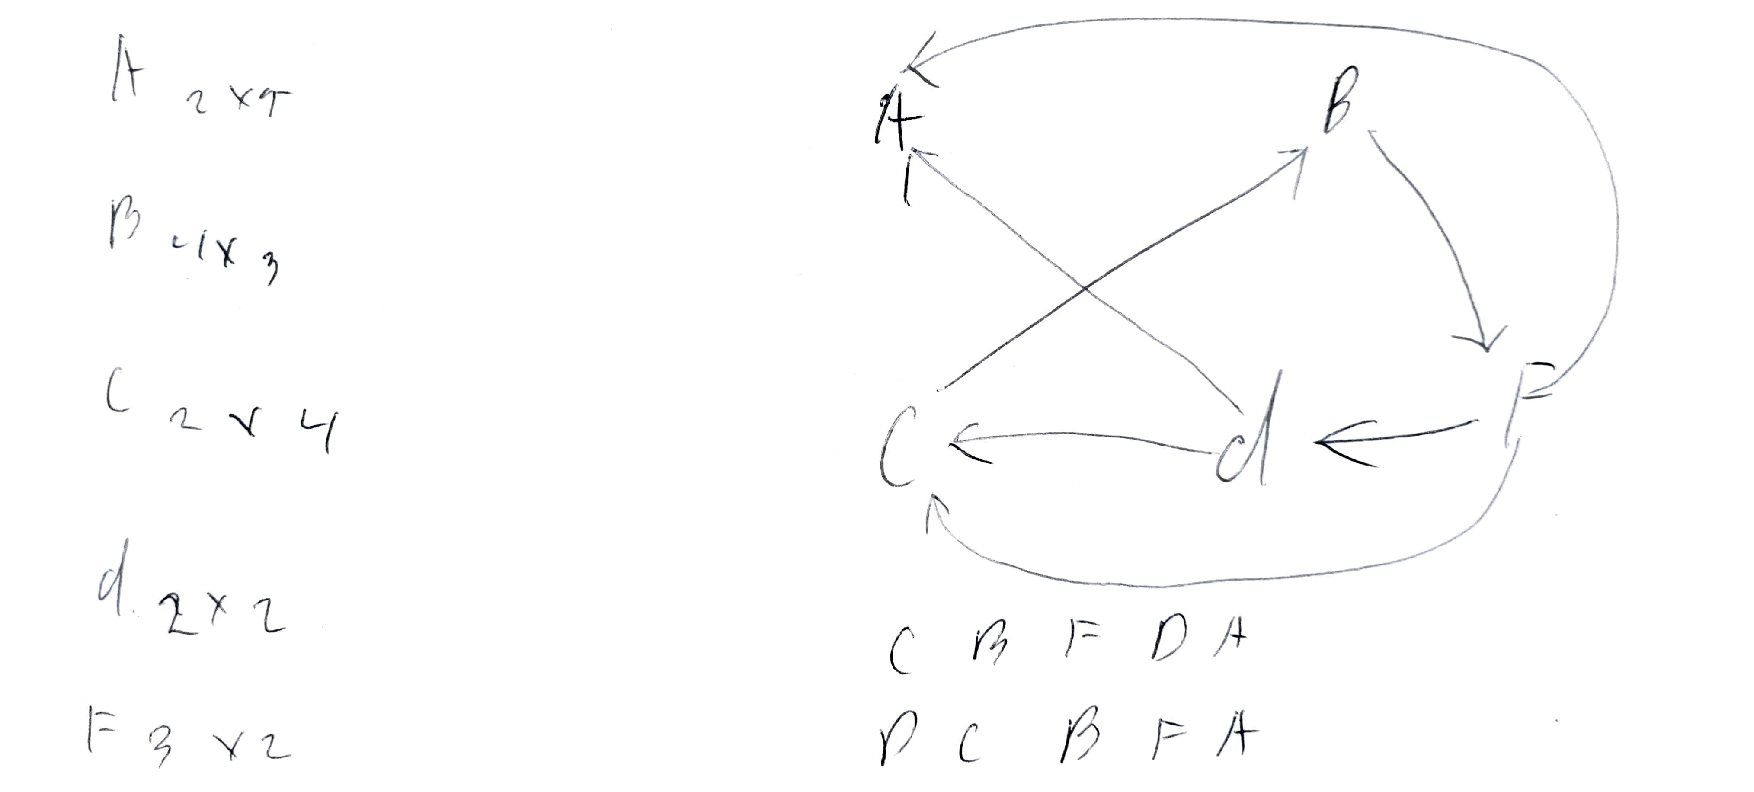
\includegraphics[width=\textwidth]{img/graph.pdf}
Исходя из того, что мы должны закончить умножение матриц, умножив справа на $A$, получим что всего возможно только 2 последовательности умножения, которые включают все матрицы: $CBFDA$ и $DCBFA$.

Запишем первое решение.

$CBFDA = \begin{pmatrix}
1 & 2 & -1 & 0\\
-3 & 0 & 1 & 2
\end{pmatrix} \begin{pmatrix}
1 & 1 & 1\\
-1 & 0 & 3\\
-2 & 1 & 4\\
0 & 0 & 3
\end{pmatrix} \begin{pmatrix}
-4 & 1\\
12 & -7\\
1 & 1
\end{pmatrix} \begin{pmatrix}
4 & -1\\
1 & 0
\end{pmatrix} \begin{pmatrix}
5 & 1 & 2 & -1 & 0\\
1 & 4 & -3 & 2 & 2
\end{pmatrix}= \begin{pmatrix}
1 & 0 & 3 \\
-5 & -2 & 7 
\end{pmatrix}  \begin{pmatrix}
-4 & 1\\
12 & -7\\
1 & 1
\end{pmatrix} \begin{pmatrix}
4 & -1\\
1 & 0
\end{pmatrix} \begin{pmatrix}
5 & 1 & 2 & -1 & 0\\
1 & 4 & -3 & 2 & 2
\end{pmatrix} =\\
\begin{pmatrix}
-1 & 4\\
3 & -12
\end{pmatrix} \begin{pmatrix}
4 & -1\\
1 & 0
\end{pmatrix} \begin{pmatrix}
5 & 1 & 2 & -1 & 0\\
1 & 4 & -3 & 2 & 2
\end{pmatrix} =\\
\begin{pmatrix}
0 & 1  \\
0 & -3  
\end{pmatrix}   \begin{pmatrix}
5 & 1 & 2 & -1 & 0\\
1 & 4 & -3 & 2 & 2
\end{pmatrix} = \begin{pmatrix}
1 & 4 & -3 & 2 & 2\\
-3 & -12 & 9 & -6 & -6
\end{pmatrix}$


$DCBFA = \begin{pmatrix}
4 & -1\\
1 & 0
\end{pmatrix} \begin{pmatrix}
1 & 2 & -1 & 0\\
-3 & 0 & 1 & 2
\end{pmatrix} \begin{pmatrix}
1 & 1 & 1\\
-1 & 0 & 3\\
-2 & 1 & 4\\
0 & 0 & 3
\end{pmatrix} \begin{pmatrix}
-4 & 1\\
12 & -7\\
1 & 1
\end{pmatrix}  \begin{pmatrix}
5 & 1 & 2 & -1 & 0\\
1 & 4 & -3 & 2 & 2
\end{pmatrix} = \begin{pmatrix}
7 & 8 & -5 & -2\\
1 & 2 & -1 & 0
\end{pmatrix} \begin{pmatrix}
1 & 1 & 1\\
-1 & 0 & 3\\
-2 & 1 & 4\\
0 & 0 & 3
\end{pmatrix} \begin{pmatrix}
-4 & 1\\
12 & -7\\
1 & 1
\end{pmatrix}  \begin{pmatrix}
5 & 1 & 2 & -1 & 0\\
1 & 4 & -3 & 2 & 2
\end{pmatrix} =\\ \begin{pmatrix}
9 & 2 & 5 \\
1 & 0 & 3
\end{pmatrix}  \begin{pmatrix}
-4 & 1\\
12 & -7\\
1 & 1
\end{pmatrix}  \begin{pmatrix}
5 & 1 & 2 & -1 & 0\\
1 & 4 & -3 & 2 & 2
\end{pmatrix}=\\ \begin{pmatrix}
-7 & 28\\
-1 & 4
\end{pmatrix}  \begin{pmatrix}
5 & 1 & 2 & -1 & 0\\
1 & 4 & -3 & 2 & 2
\end{pmatrix}= \begin{pmatrix}
-7 & 105 & -98 & 63 & 56\\
-1 & 15 & -14 & 9 & 8
\end{pmatrix}$

\textbf{Ответ: два варианта перемножения $CBFDA = \begin{pmatrix}
1 & 4 & -3 & 2 & 2\\
-3 & -12 & 9 & -6 & -6
\end{pmatrix}$ и $DCBFA = \begin{pmatrix}
-7 & 105 & -98 & 63 & 56\\
-1 & 15 & -14 & 9 & 8
\end{pmatrix}$}

\vspace{5pt}

\item Пусть $A\in M_n(\mathbb{R})$ такова, что $A^m = 0$ для некоторого натурального $m$. Покажите, что матрица $(E - A)$ обратима ({\it указание: найдите явный вид обратной матрицы}).

\textbf{Решение:}\\
Догадаемся, что можно соорудить конструкцию, похожую на сумму бесконечной геометрической прогрессии. По аналогии с $\frac{1}{1-x} \sim (E-A)^-1$
$$(E-A)^-1=\sum^{\infty}_{m=0}A^m=E+A+A^2 + A^3+\ldots + A^{m-1}+A^{m}+\ldots $$
При этом $A^m = 0$ и все слагаемые с большим $m$ будут равны 0, следовательно сумма будет выглядеть.
$$(E-A)^-1=\sum^{m-1}_{m=0}A^m=E+A+A^2 + A^3+\ldots + A^{m-1}$$

Проверим, что будет при перемножении этой матрицы на исходную.
$$(E-A)(E-A)^-1=(E-A)\sum^{m-1}_{m=0}A^m=(E-A)(E+A+A^2 + A^3+\ldots + A^{m-1})=$$$$=E+A+A^2 + A^3+\ldots + A^{m-1}-A-A^2 + A^3-\ldots - A^{m-1}-A^{m} = E-A^m + \sum_{i=1}^{m-1}{A^i-A^i}$$
так как $A^m = 0$, то сумма сверху = $E-0+0=E$, следовательно мы получили формулу для обратной матрицы

\textbf{Ответ: обратную матрицу к можно найти таким образом: $(E-A)^-1=\sum^{m-1}_{m=0}A^m=E+A+A^2 + A^3+\ldots + A^{m-1}$}

\vspace{5pt}


\end{enumerate}
\end{document}